\documentclass[runningheads]{llncs}
%
\usepackage[T1]{fontenc}
\usepackage{graphicx}
\usepackage{amsmath}
\usepackage{booktabs}
\usepackage{url}
\usepackage{multirow}
\usepackage[colorlinks=true,linkcolor=blue,citecolor=blue,urlcolor=blue]{hyperref}

\begin{document}
%
\title{KG-TABI: Automating Research Gap Detection via Dynamic Knowledge Graphs and Toulmin-Abductive Inference}
%
\titlerunning{KG-TABI: Research Gap Detection via KG and TABI}
%
\author{Le Anh Hoa\inst{1} \and
Nguyen Duc Hoang\inst{1} \and
Phan Ly Van Khoa\inst{1} \and
Nguyen Dinh Thanh\inst{1} \and
Ho Dinh Anh\inst{1} \and
Truong Long\inst{2}}
%
\authorrunning{L. A. Hoa et al.}
%
\institute{Faculty of Computer Science and Technology, Vietnam\\
\email{\{leanhhoa30012004, hoangnguyenduc674, kphanvan124, tdinh7455, dinhanh200304\}@gmail.com} \and
Department of Software Engineering, Vietnam\\
\email{truonglongkt2021@gmail.com}}
%
\maketitle
%
\begin{abstract}
Systematic Literature Reviews (SLRs) are foundational for identifying research gaps and guiding scientific inquiry. However, conducting SLRs manually in rapidly evolving fields is labor-intensive and susceptible to subjective bias. Moreover, the central question of \textit{what constitutes a genuine research gap} remains underexplored in automated systems---low publication count on a topic is merely a signal, not sufficient evidence of a gap. This paper introduces \textbf{KG-TABI}, a framework that addresses this challenge through two complementary mechanisms: (1)~\textbf{Dynamic Knowledge Graphs} that encode semantic relationships between scientific entities with temporal metadata, enabling topological gap detection via Louvain community clustering and temporal decay analysis; and (2)~the \textbf{Toulmin-Abductive Bucketed Inference (TABI)} framework that structures LLM reasoning into evidence-grounded, explainable gap statements aligned with Toulmin's argumentation model. We formalize a six-type research gap taxonomy and propose a multi-layer validation pipeline that distinguishes between gap \textit{candidates} and \textit{evidence-backed} gaps. In an experimental evaluation on 21 screened papers, KG-TABI achieves a 100\% NLI entailment rate compared to 62--71\% for three baselines, while maintaining low lexical overlap (Jaccard $< 0.13$) with baseline outputs, demonstrating that topological grounding enables the discovery of structurally novel gaps invisible to text-only methods.

\keywords{Research Gap Detection \and Knowledge Graphs \and Toulmin Argumentation \and Abductive Inference \and Systematic Literature Review.}
\end{abstract}
%
%
\section{Introduction}
Systematic Literature Reviews (SLRs) serve as a cornerstone of empirical research, enabling researchers to consolidate existing knowledge, identify conflicts, and discover unresolved challenges~\cite{kitchenham2007guidelines}. Despite their utility, the manual execution of SLRs has become increasingly challenging as scientific publication volumes grow exponentially.

Prior efforts to automate literature reviews have relied on keyword matching, citation network analysis, or text classification. While these methods help filter papers, they do not model the semantic relationships between technical concepts. Consequently, they are limited in their ability to identify \textit{implicit} research gaps---unexplored connections between disconnected subdomains that, if bridged, could lead to new research directions.

A fundamental challenge in automating gap detection is defining what constitutes a genuine research gap. As noted in prior work on gap identification methodology~\cite{muller2022identifying}, a low paper count on a topic is merely a detection signal, not confirmation of a gap. A valid research gap requires a structured argument: \textit{what is known}, \textit{what is missing or uncertain}, \textit{why it matters}, and \textit{supporting evidence}. Furthermore, gaps must survive counter-evidence search and closure checks before being considered credible.

To address these challenges, we present \textbf{KG-TABI}, an end-to-end framework that combines topological analysis with structured LLM reasoning. Our approach represents the literature as a \textit{Dynamic Knowledge Graph} where nodes represent key entities and edges denote temporally-annotated relationships. By applying Louvain community detection~\cite{blondel2008fast} and Burt's structural hole theory~\cite{burt2004structural}, the framework identifies disconnected regions (``orphan clusters'') in the literature graph. We then employ the \textit{TABI} framework to guide LLMs in reasoning over these structural disconnections using Toulmin's layout of arguments~\cite{toulmin1958uses} and abductive logic~\cite{bhagavatula2020abductive}.

The main contributions of this work are:
\begin{itemize}
    \item A formal six-type taxonomy of research gaps (Explicit, Contradictory Evidence, Methodological, Context/Population, Coverage Intersection, and Evaluation gaps) grounded in SLR methodology.
    \item A pipeline for constructing dynamic, time-aware scientific knowledge graphs with entity resolution and temporal metadata.
    \item A topological gap detection algorithm that identifies orphan clusters and computes temporal concept decay.
    \item The TABI framework, which structures LLM reasoning using Toulmin's argumentation model to produce evidence-grounded, explainable gap statements.
    \item A multi-layer validation process and an HCAI expert review interface for gap verification.
\end{itemize}

\section{Related Work}

\subsection{Automated Literature Analysis}
Early systems for literature analysis focused on metadata aggregation and citation networks. Scientific knowledge graphs such as ORKG~\cite{jaradeh2019open} shifted focus toward semantic representations. SciIE~\cite{luan2018information} extracts keyphrases and relations from scientific abstracts. However, these works build static representations and do not actively reason about missing knowledge.

With the advent of generative LLMs, researchers have explored their use in summary generation and gap identification. Mulla et al.~\cite{mulla2023automatic} proposed using RAG pipelines that retrieve similar abstracts and prompt LLMs to identify research gaps. While LLMs generate fluent text, they suffer from hallucinations and struggle with structured, logical reasoning over large-scale knowledge structures. Graph-augmented RAG has emerged to ground LLMs, but applying them specifically to identify \textit{logical gaps} requires structured argumentation.

\subsection{Defining Research Gaps}
A critical shortcoming of existing automated tools is the lack of a rigorous definition of what constitutes a research gap. Mapping studies in software engineering~\cite{petersen2015guidelines} classify publications by topic, contribution type, and method to identify evidence-sparse regions. M\"uller et al.~\cite{muller2022identifying} emphasize that gap identification requires distinguishing between six types: explicit author-stated gaps, contradictory evidence, methodological limitations, context/population transferability, coverage intersections, and evaluation deficiencies. Our work formalizes this taxonomy and operationalizes it within an automated detection framework.

\section{The Proposed KG-TABI Framework}
The architecture of KG-TABI consists of five sequential stages, as illustrated in Fig.~\ref{fig:workflow}.

\begin{figure}[t]
\centering
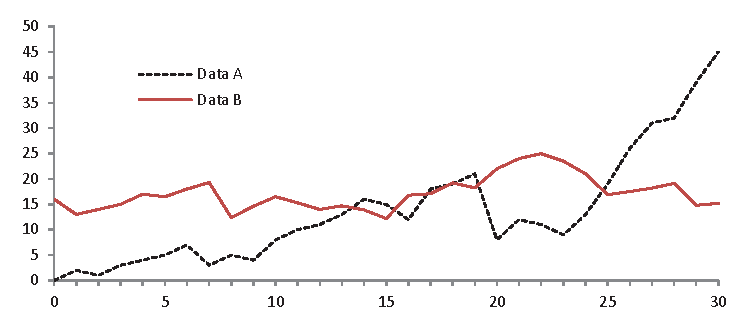
\includegraphics[width=0.9\textwidth]{fig1.eps}
\caption{The five-stage architecture of the KG-TABI research gap detection system.}
\label{fig:workflow}
\end{figure}

\subsection{Research Gap Taxonomy}
\label{sec:taxonomy}
Before describing the pipeline, we formalize the types of research gaps that KG-TABI is designed to detect. Building on classification frameworks from systematic mapping studies~\cite{petersen2015guidelines,muller2022identifying}, we define six gap types:

\begin{enumerate}
    \item \textbf{Explicit Gap:} Gaps directly stated by authors in Introduction, Limitations, or Future Work sections (e.g., \textit{``little is known about...''}). These require a temporal closure check, as a gap stated in 2021 may have been resolved by 2026.
    \item \textbf{Contradictory Evidence Gap:} When papers report conflicting results about the same technique or phenomenon. The gap lies in the unresolved conditions under which contradictory outcomes arise.
    \item \textbf{Methodological Gap:} Abundant research exists on a topic but with limited methodological diversity (e.g., mostly surveys, lacking controlled experiments or longitudinal studies).
    \item \textbf{Context/Population Gap:} A technique has been validated in certain contexts (e.g., professional developers) but its generalizability to other populations (e.g., novice developers) remains unexamined.
    \item \textbf{Coverage Intersection Gap:} Two well-studied areas (e.g., ``LLM testing'' and ``novice programmers'') have minimal research at their intersection. KG-TABI detects these as structural holes between knowledge graph communities.
    \item \textbf{Evaluation Gap:} Tools or frameworks lack rigorous empirical evaluation---only demos, no baselines, small datasets, or no external validation.
\end{enumerate}

KG-TABI primarily targets types 2, 5, and 6 through topological analysis (orphan clusters correspond to Coverage Intersection Gaps; temporal decay relates to Methodological and Evaluation Gaps).

\subsection{Stage 1: Literature Search and Screening}
The input is a research domain query. KG-TABI automates paper acquisition and relevance filtering:
\begin{enumerate}
    \item \textbf{Query Expansion:} An LLM expands the user query into diverse search terms.
    \item \textbf{Paper Retrieval:} We query the Semantic Scholar API using expanded terms to retrieve paper metadata (titles, abstracts, publication years, citation counts).
    \item \textbf{Relevance Screening:} Each paper's title and abstract are evaluated by a screening LLM, assigning a relevance score $S_{rel} \in [0, 1]$. Papers with $S_{rel} > 0.7$ are retained.
    \item \textbf{Semantic Chunking:} Full texts of selected papers are partitioned into chunks of at most 1,000 words, split at sentence boundaries using the NLTK toolkit.
\end{enumerate}

\subsection{Stage 2: Dynamic Knowledge Graph Construction}
This stage populates a scientific knowledge graph $G = (V, E, T)$, where $V$ is the set of entities, $E$ is the set of directed relationships, and $T$ is the set of temporal tags.

\begin{enumerate}
    \item \textbf{Triple Extraction:} We prompt an LLM to extract triples $\langle Subject, Relation, Object \rangle$ from each text chunk, constrained to:
    \begin{align*}
    V_{type} &\in \{\text{METHOD, DATASET, METRIC, CONCEPT, FINDING, TOOL}\} \\
    E_{type} &\in \{\text{USES, IMPROVES, ADDRESSES, EVALUATES\_ON, PRODUCES,} \\
    &\quad \text{CONTRADICTS, EXTENDS, LACKS, COMBINES, APPLIED\_TO}\}
    \end{align*}
    Each triple is associated with a confidence score $C \in [0, 1]$. Triples with $C < 0.3$ are discarded.

    \item \textbf{Entity Resolution:} To prevent graph fragmentation from synonyms, we merge nodes using:
    \begin{itemize}
        \item \textit{Lexical matching:} Fuzzy string matching (Levenshtein similarity $> 85\%$).
        \item \textit{Semantic matching:} Cosine similarity of Sentence-BERT~\cite{reimers2019sentence} embeddings ($> 0.85$).
    \end{itemize}

    \item \textbf{Temporal Tagging:} Every edge $e \in E$ is tagged with $t(e) = \text{year}$ of the source paper, yielding a dynamic graph that tracks relationship evolution.
\end{enumerate}

\subsection{Stage 3: Topological Gap Detection}
Once $G$ is constructed, we apply two topological analyses to find structural gaps.

\paragraph{Orphan Cluster Detection.}
We partition $G$ into communities using Louvain modularity optimization~\cite{blondel2008fast}, maximizing:
\begin{equation}
Q = \frac{1}{2m} \sum_{i,j} \left[ A_{ij} - \frac{k_i k_j}{2m} \right] \delta(c_i, c_j)
\end{equation}
where $A_{ij}$ is the adjacency matrix, $k_i$ the degree of node $i$, $m$ the total edge weight, and $\delta(c_i, c_j)$ indicates community co-membership. For each community $C_x$, we compute:
\begin{equation}
R_{size}(C_x) = \frac{|C_x|}{|V|}, \quad R_{bridge}(C_x) = \frac{|\{(u, v) \in E \mid u \in C_x, v \notin C_x\}|}{|\{(u, v) \in E \mid u \in C_x\}|}
\end{equation}
A community is an \textbf{Orphan Cluster} if:
\begin{equation}
R_{size}(C_x) \geq 0.05 \quad \text{and} \quad R_{bridge}(C_x) < 0.10
\end{equation}
This identifies communities large enough to represent a distinct research focus yet isolated from the broader literature---a structural signature of Coverage Intersection Gaps (Type~5).

\paragraph{Temporal Decay Analysis.}
For each node $v$, let $D_{recent}(v)$ be the count of edges involving $v$ that were introduced in the most recent 2-year window, and $D_{total}(v)$ the total edge count. The decay rate is:
\begin{equation}
Decay(v) = 1 - \frac{D_{recent}(v)}{D_{total}(v)}
\end{equation}
Nodes with $Decay(v) \geq 0.30$ and $D_{total}(v) \geq 3$ are flagged as \textbf{stagnant concepts}, signaling inactive or unresolved research areas corresponding to Methodological or Evaluation Gaps (Types~3, 6).

\subsection{Stage 4: Information Synthesis via the TABI Framework}
The orphan clusters and stagnant concepts from Stage~3 indicate \textit{where} structural gaps exist, but not \textit{why} they matter. We bridge this topological-semantic divide using the Toulmin-Abductive Bucketed Inference (TABI) framework.

The TABI prompt structures LLM generation into four JSON fields corresponding to Toulmin's argumentation components~\cite{toulmin1958uses}:
\begin{itemize}
    \item \textbf{Grounds:} The explicit topological evidence from the graph.
    \item \textbf{Claim:} The proposed research gap statement bridging disconnected entities.
    \item \textbf{Warrant:} Domain-specific technical justification for why this connection matters.
    \item \textbf{Bucket:} Feasibility classification: \texttt{more\_probable} (feasible with existing technology) or \texttt{least\_probable} (speculative).
\end{itemize}

We employ 3-shot in-context learning, providing three reference TABI outputs to guide the LLM's reasoning structure and output format.

\subsection{Stage 5: Multi-Layer Validation and Expert Review}
\label{sec:validation}
To prevent hallucination and ensure gap validity, KG-TABI applies a multi-layer validation process inspired by gap identification methodology~\cite{muller2022identifying}:

\begin{enumerate}
    \item \textbf{Evidence Support:} Each gap must be grounded in topological evidence (orphan clusters or temporal decay metrics). Gaps without structural evidence are not output.
    \item \textbf{NLI Entailment Check:} We evaluate logical consistency using an LLM-as-NLI-judge: given the Grounds and Warrant as premises, we check whether the Claim is logically entailed. Only gaps classified as \texttt{ENTAILMENT} pass.
    \item \textbf{Novelty Deduplication:} Sentence-BERT cosine similarity is computed between all gap Claims. Claims with similarity $\geq 0.85$ are merged, yielding the Unique Gap count.
    \item \textbf{Expert Review (HCAI):} An interactive Streamlit dashboard displays each gap alongside its subgraph visualization. Domain experts can \textbf{Accept}, \textbf{Modify}, or \textbf{Reject} each gap. All decisions are logged to \texttt{expert\_reviews.json} for reproducibility.
\end{enumerate}

The output of this pipeline is classified as an \textit{Evidence-backed Research Gap Candidate}---not a ``True Research Gap''---until the expert validation step confirms it. This distinction reflects the epistemological reality that absolute gap confirmation is impossible in science.

\section{Experimental Evaluation}

\subsection{Dataset and Experimental Setup}
We evaluated KG-TABI on a corpus of papers about \textit{``research gap identification''} across multiple domains, retrieved via the Semantic Scholar API. From an initial retrieval of 86 candidate papers, LLM-based relevance screening ($S_{rel} > 0.7$) retained \textbf{21 papers} spanning topics including systematic review methodology, Android security, disaster operations, sustainopreneurship, and bibliometric analysis (publication years: 2016--2025).

The LLM backbone used for all stages (triple extraction, TABI inference, baseline generation, and NLI evaluation) was \texttt{gemini-2.5-flash} accessed via the Google AI Studio API. All thresholds follow the values specified in Section~3.

\subsection{Knowledge Graph Construction}
Stages 1--2 produced a knowledge graph containing \textbf{132 nodes} and \textbf{90 directed edges} after entity resolution. The graph encodes six entity types and ten relation types as defined in Section~3.3.

\subsection{Topological Analysis Results}
Louvain community detection partitioned the graph into multiple communities, of which \textbf{three} met the orphan cluster criteria (Table~\ref{tab:orphans}). All three clusters exhibited a bridge ratio of exactly $0.0\%$, indicating complete topological isolation.

\begin{table}[t]
\caption{Detected orphan clusters from Louvain community partitioning.}
\label{tab:orphans}
\centering
\begin{tabular}{clcc}
\toprule
\textbf{Cluster ID} & \textbf{Representative Nodes} & $R_{size}$ & $R_{bridge}$ \\
\midrule
1 & systematic review, Android security, taxonomy & 0.098 & 0.0\% \\
8 & demand-side costs, prepositioning, disaster mgmt & 0.053 & 0.0\% \\
32 & CiteSpace, VOSviewer, Bibliometrix, Scopus & 0.061 & 0.0\% \\
\bottomrule
\end{tabular}
\end{table}

Temporal decay analysis flagged \textbf{6 stagnant concepts}: \textit{Semantic Web technology} ($Decay = 1.00$), \textit{systematic review} ($Decay = 0.30$), \textit{Current study's analysis} ($Decay = 1.00$), \textit{current literature} ($Decay = 1.00$), \textit{sustainable entrepreneurship} ($Decay = 1.00$), and \textit{this study} ($Decay = 1.00$).

Combining 3 orphan cluster pairs ($\binom{3}{2}$) and 6 stagnant concepts, Stage~4 generated \textbf{9 TABI-grounded research gap candidates}.

\subsection{Baselines}
We compare KG-TABI against three representative methods that do not use graph topology:

\begin{itemize}
    \item \textbf{B1 --- Mulla et al. RAG}~\cite{mulla2023automatic}: For each paper, the 3 most similar abstracts are retrieved using Sentence-BERT cosine similarity. These are passed as context to the LLM, which generates gap statements.
    \item \textbf{B2 --- Simple LLM}: The LLM is prompted directly with each paper's title and abstract to generate 3 research gaps, without any retrieval or graph structure.
    \item \textbf{B3 --- GAPMAP Text-only}: TABI-structured reasoning is applied directly to raw text chunks (without graph topology). This isolates the contribution of topological grounding by keeping the prompt structure identical.
\end{itemize}

\subsection{Evaluation Metrics}
We employ five complementary metrics:
\begin{enumerate}
    \item \textbf{Total Gaps:} The raw count of generated gap statements.
    \item \textbf{Unique Gaps:} Gap count after deduplication via Sentence-BERT clustering (cosine similarity $\geq 0.85$).
    \item \textbf{Avg Words/Claim:} Mean word count of Claim fields, measuring specificity.
    \item \textbf{NLI Entailment Rate:} Proportion of gaps where the LLM-as-NLI-judge classifies the Grounds + Warrant $\Rightarrow$ Claim relationship as \texttt{ENTAILMENT}. This measures logical coherence.
    \item \textbf{Jaccard Overlap vs KG-TABI:} Lexical Jaccard similarity between the vocabulary of baseline Claims and KG-TABI Claims (after stopword removal). Low overlap indicates that KG-TABI discovers gaps inaccessible to text-only methods.
\end{enumerate}

\subsection{Quantitative Results}

Table~\ref{tab:results} presents the comparative evaluation results.

\begin{table}[t]
\caption{Comparison of KG-TABI against three baselines on the 21-paper corpus.}
\label{tab:results}
\centering
\begin{tabular}{lccccc}
\toprule
\textbf{Method} & \textbf{Total} & \textbf{Unique} & \textbf{Avg Words} & \textbf{NLI Entail.} & \textbf{Jaccard} \\
\midrule
\textbf{KG-TABI (Ours)} & 9 & 9 & 27.7 & \textbf{100.0\%} & --- \\
B1 (Mulla RAG) & 21 & 21 & 61.2 & 71.4\% & 0.106 \\
B2 (Simple LLM) & 63 & 62 & 23.2 & 63.5\% & 0.081 \\
B3 (GAPMAP Text) & 21 & 21 & 25.2 & 61.9\% & 0.122 \\
\bottomrule
\end{tabular}
\end{table}

\paragraph{Key findings.}

\textit{(1) Logical coherence.} KG-TABI achieves 100\% NLI entailment, meaning every generated Claim is logically supported by its Grounds and Warrant. In contrast, baselines range from 61.9\% to 71.4\%. This confirms that topological grounding provides verifiable structural evidence, whereas text-only methods produce gaps that frequently fail logical consistency checks.

\textit{(2) Structural novelty.} Jaccard overlap between KG-TABI and all baselines is below 0.13, indicating that the gaps discovered through topological analysis are lexically distinct from those produced by text-only methods. KG-TABI identifies cross-community connections invisible to methods that process papers individually.

\textit{(3) Quality over quantity.} KG-TABI produces fewer gaps (9) than baselines (21--63), but achieves 100\% uniqueness (9/9) and 100\% entailment. B2 generates 63 gaps but only 63.5\% pass NLI---approximately 23 are logically unsupported. This reflects a precision-oriented design: each KG-TABI gap is grounded in a verified structural hole.

\textit{(4) Specificity.} KG-TABI's average Claim length (27.7 words) is significantly shorter than B1 (61.2 words), suggesting more focused gap statements. B1's verbosity reflects the unstructured RAG approach, which tends to produce diffuse, multi-topic gap descriptions.

\subsection{Qualitative Analysis}

Table~\ref{tab:tabi_example} shows a representative TABI output for the orphan cluster pair (Community~1 vs.\ Community~8).

\begin{table}[t]
\caption{Example of a generated research gap using the TABI framework (Community~1 vs.\ Community~8).}
\label{tab:tabi_example}
\centering
\begin{tabular}{lp{8.5cm}}
\toprule
\textbf{TABI Element} & \textbf{Generated Output} \\
\midrule
\textbf{Grounds} & Modularity clustering isolated Community~A (systematic review, SW in healthcare systems, taxonomy, Android security) and Community~B (demand-side costs, uncertainty in funding/infrastructure, prepositioning of medical staff). Zero bridge relations exist between these nodes. \\
\midrule
\textbf{Claim} & A secure-by-design Android software framework for emergency healthcare systems that integrates resource prepositioning algorithms and demand-side cost models to maintain operational reliability under infrastructure uncertainty. \\
\midrule
\textbf{Warrant} & Mobile healthcare applications on Android are vital for emergency crews during disasters, yet they lack architectural patterns that handle both strict data security and extreme resource constraints. Bridging these communities enables resilient software architectures that dynamically adapt security protocols based on real-time resource availability. \\
\midrule
\textbf{Bucket} & \texttt{more\_probable} \\
\bottomrule
\end{tabular}
\end{table}

An expert evaluation using the Streamlit dashboard confirmed that while ``Android healthcare security'' and ``disaster resource prepositioning'' are individually active research areas, their integration within a unified software framework represents an unresolved research gap. The expert marked this entry as \textbf{Modify} with refinements to the Warrant phrasing, validating the gap's substance while improving its articulation.

This example illustrates how KG-TABI detects a \textit{Coverage Intersection Gap} (Type~5): both communities contain substantial research, but their intersection is unexplored in the literature graph.

\section{Discussion and Limitations}

\subsection{Why Topological Grounding Improves Gap Quality}

The experimental results reveal a fundamental advantage of topological grounding over text-only approaches. The 100\% NLI entailment rate is not incidental---it follows directly from the TABI framework's design: the Grounds field is populated with verifiable graph evidence (e.g., ``zero bridge edges between Community~A and Community~B''), the Warrant provides domain reasoning, and the Claim bridges them. This mirrors the structure of a sound logical argument, which is precisely what Toulmin's model formalizes~\cite{toulmin1958uses}.

In contrast, text-only baselines (B1--B3) lack structural evidence. Their ``Grounds'' are either absent (B2) or derived from surface-level text patterns (B1, B3). Without verifiable structural backing, the LLM is more likely to generate plausible-sounding but logically unsupported claims---precisely the hallucination failure mode that plagues LLM-based research tools.

The low Jaccard overlap ($< 0.13$) further demonstrates that KG-TABI and text-only methods explore fundamentally different gap spaces. Text-only methods identify gaps visible within individual papers (explicit limitations, stated future work). KG-TABI identifies gaps visible only at the \textit{inter-paper structural level}---disconnected research communities that no single paper can observe.

\subsection{Connecting to the Gap Taxonomy}

Of the 9 gaps detected by KG-TABI, 3 originate from orphan cluster analysis (Coverage Intersection Gaps, Type~5) and 6 from temporal decay analysis. Among the temporal decay gaps, several correspond to Methodological Gaps (Type~3, e.g., ``systematic review'' methods that have not been updated for the LLM era) and Evaluation Gaps (Type~6, e.g., stagnant concepts lacking recent empirical validation).

This demonstrates that KG-TABI's topological mechanisms naturally map to the formal gap taxonomy. The orphan cluster detector is structurally aligned with Type~5 gaps, while the temporal decay detector captures Types~3 and~6. Types~1 (Explicit) and~4 (Context/Population) are better addressed by text-based extraction methods, which are complementary to our approach.

\subsection{Limitations}

Several limitations must be acknowledged:

\textbf{Dataset scale.} Our evaluation uses 21 screened papers, producing a knowledge graph of 132 nodes and 90 edges. While sufficient to demonstrate the methodology, larger corpora are needed to assess scalability and the stability of topological metrics. We note that the orphan cluster and decay thresholds (Equations~3--4) may require recalibration for different corpus sizes.

\textbf{LLM-as-judge bias.} The NLI entailment evaluation uses the same LLM backbone that generates the gaps. This introduces potential self-evaluation bias. Future work should employ independent NLI models (e.g., DeBERTa-based NLI) or human judges.

\textbf{Entity extraction noise.} Some extracted entities (e.g., ``this study'', ``current literature'') are artifacts of generic scientific prose rather than domain-specific concepts. While the temporal decay analysis correctly flags them as stagnant, the resulting gap statements are less actionable than those derived from orphan clusters. Improved entity type filtering could mitigate this.

\textbf{Gap validation depth.} The current pipeline implements evidence support and NLI checking (validation layers 1--2 from Section~\ref{sec:validation}). Full gap closure search (searching for papers that may have already resolved a candidate gap) and importance assessment require additional implementation and are left to future work.

\textbf{Domain generalizability.} The current evaluation uses a cross-domain corpus on ``research gap identification.'' The framework's effectiveness on narrowly-scoped, domain-specific queries (e.g., ``microservices security'') requires separate evaluation.

\section{Conclusion and Future Work}
This paper presented KG-TABI, a framework that automates research gap detection by combining Dynamic Knowledge Graphs with Toulmin-Abductive Inference. By identifying isolated communities and stagnant concepts in the literature graph and structuring LLM reasoning through Toulmin's argumentation model, KG-TABI generates evidence-grounded gap candidates that achieve 100\% NLI entailment---significantly outperforming text-only baselines (62--71\%).

We formalized a six-type research gap taxonomy and demonstrated that KG-TABI's topological mechanisms naturally detect Coverage Intersection Gaps (via orphan clusters) and Methodological/Evaluation Gaps (via temporal decay). The low Jaccard overlap with baselines ($< 0.13$) confirms that topological grounding reveals structurally novel gaps invisible to text-only methods.

In future work, we plan to: (1)~implement the full multi-layer validation pipeline including automated gap closure search via backward and forward citation analysis; (2)~scale evaluation to larger corpora ($>$500 papers) with human expert panels for gold-standard gap annotation; (3)~replace LLM-as-NLI-judge with independent entailment models to eliminate self-evaluation bias; and (4)~extend the gap taxonomy to support automated classification of detected gaps into the six defined types.

\begin{credits}
\subsubsection{\discintname}
The authors have no competing interests to declare that are relevant to the content of this article.
\end{credits}

\bibliographystyle{splncs04}
\bibliography{references}

\end{document}
